% no answer key
\documentclass[letterpaper]{exam}

% answer key
% \documentclass[letterpaper, landscape]{exam}
% \usepackage{2in1, lscape} 
% \printanswers

\usepackage{units} 
\usepackage{xfrac} 
\usepackage[fleqn]{amsmath}
\usepackage{float}
\usepackage{mdwlist}
\usepackage{booktabs}
\usepackage{cancel}
\usepackage{polynom}
\usepackage{caption}
\usepackage{fullpage}
\usepackage{comment}
\usepackage{enumerate}
\usepackage{graphicx}

\usepackage{mathtools} 

\newcommand{\dg}{\ensuremath{^\circ}} 
\newcommand{\sgn}{\operatorname{sgn}}

\everymath{\displaystyle}
\title{Calculus I \\ Homework Eight \\ Section 2.8}
\author{}
\date{\today}

\begin{document}

  \maketitle

  \section{Homework}
    \begin{itemize*}
      \item read Section 2.8
      \item exercises: 1, 3-9, 14, 19-28, 35-37, 41-43
    \end{itemize*}

  \ifprintanswers

  \section{Solutions}

    \begin{description}

      \item[1] 
        \begin{enumerate}[(a)]
          \item $f'(-3) \approx 1$
          \item $f'(-2) \approx 1$
          \item $f'(-1) \approx 0$
          \item $f'(0) \approx -4$
          \item $f'(1) \approx 0$
          \item $f'(2) \approx 1$
          \item $f'(3) \approx 1$
        \end{enumerate}

      \newpage

      \item[3] 
        \begin{enumerate}[(a)]
          \item \fbox{ II }
          \item \fbox{ IV }
          \item \fbox{ I }
          \item \fbox{ III }
        \end{enumerate}

      \item[4-9] graphs

      \item[14]
        The derivative of $\sin(x)$ looks like $\cos(x)$. See Figure \ref{fig:ex14}.

        \begin{figure}[H]
          \centering
          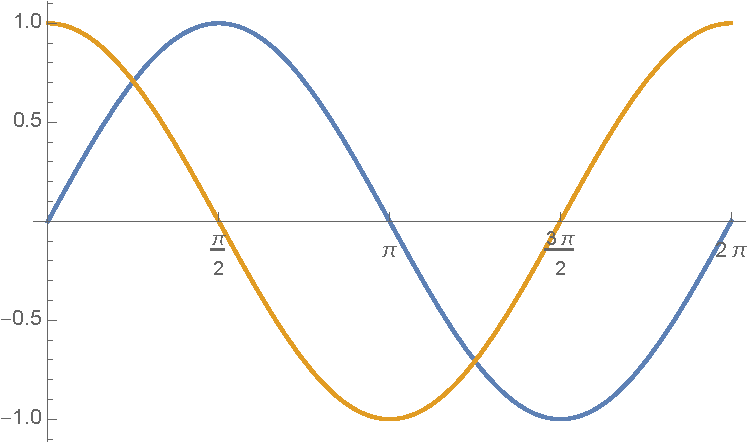
\includegraphics[scale = 0.5]{ex14.pdf}
          \caption{Exercise 15}
          \label{fig:ex14}
        \end{figure}

      \item[19]
        \begin{itemize}
          \item $f'(x) = \frac{1}{2}$
          \item Domain $f$: $(-\infty, \infty)$
          \item Domain $f'$: $(-\infty, \infty)$
        \end{itemize}

      \item[20]
        \begin{itemize}
          \item $f'(x) = m$
          \item Domain $f$: $(-\infty, \infty)$
          \item Domain $f'$: $(-\infty, \infty)$
        \end{itemize}

      \item[21]
        \begin{itemize}
          \item $f'(t) = -18t + 5$
          \item Domain $f$: $(-\infty, \infty)$
          \item Domain $f'$: $(-\infty, \infty)$
        \end{itemize}

      \newpage

      \item[22]
        \begin{itemize}
          \item $f'(x) = 3x - 1$
          \item Domain $f$: $(-\infty, \infty)$
          \item Domain $f'$: $(-\infty, \infty)$
        \end{itemize}

      \item[23]
        \begin{itemize}
          \item $f'(x) = 3x^2 - 3$
          \item Domain $f$: $(-\infty, \infty)$
          \item Domain $f'$: $(-\infty, \infty)$
        \end{itemize}

      \item[24]
        \begin{itemize}
          \item $f'(x) = 1 + \frac{1}{ 2 \sqrt{x} }$
          \item Domain $f$: $[ 0, \infty )$
          \item Domain $f'$: $( 0, \infty )$
        \end{itemize}

      \item[25]
        \begin{itemize}
          \item $f'(x) = \frac{1}{\sqrt{1 + 2x}}$
          \item Domain $f$: $\left[ - \frac{1}{2}, \infty \right)$
          \item Domain $f'$: $\left( - \frac{1}{2}, \infty \right)$
        \end{itemize}

      \item[26]
        \begin{itemize}
          \item $f'(x) = \frac{10}{(1 - 3x)^2}$
          \item Domain $f$: $x \neq \frac{1}{3}$
          \item Domain $f'$: $x \neq \frac{1}{3}$
        \end{itemize}

      \item[27]
        \begin{itemize}
          \item $f'(t) = \frac{4}{(t + 1)^2}$
          \item Domain $f$: $t \neq -1$
          \item Domain $f'$: $t \neq -1$
        \end{itemize}

      \item[28]
        \begin{itemize}
          \item $f'(t) = -\frac{ 1 }{ 2t^{3/2} }$
          \item Domain $f$: $(0, \infty)$
          \item Domain $f'$: $(0, \infty)$
        \end{itemize}

      \item[35] 
        \begin{itemize*}
          \item $x = -4$
          \item $x = 0$
        \end{itemize*}

      \item[36] 
        \begin{itemize*}
          \item $x = 0$
          \item $x = 3$
        \end{itemize*}

      \item[37] 
        \begin{itemize*}
          \item $x = -1$
          \item $x = 4$
        \end{itemize*}

      \item[41] 
        \begin{enumerate}[(a)]
          \item $f$
          \item $f'$ $b$ is the slope of $a$
          \item $f''$ $c$ is the slope of $b$
        \end{enumerate}

      \item[42] 
        \begin{enumerate}[(a)]
          \item $f'''$ $a$ is the slope of $b$
          \item $f''$ $b$ is the slope of $c$
          \item $f'$ $c$ is the slope of $d$
          \item $f$ 
        \end{enumerate}

      \item[43]
        \begin{enumerate}[(a)]
          \item acceleration: slope of velocity
          \item velocity: slope of position
          \item position
        \end{enumerate}

     \end{description}
 
  \else
    \vspace{10 cm}
    \begin{quote}
      \begin{em}
        Do you see law and order? There is nothing but disorder, and instead of law there
        is the illusion of security. It is an illusion because it is built on a long
        history of injustices: racism, criminality, and the genocide of millions. Many
        people say it is insane to resist the system, but actually, it is insane not to. 
      \end{em}
    \end{quote}
    \hspace{2 cm} --Mumia Abu-Jamal
  \fi

\end{document}

